\documentclass[11pt,a4paper]{article}

% Packages
\usepackage{amsmath}
\usepackage{amssymb}
\usepackage{amsthm}
\usepackage[margin=1in]{geometry}
\usepackage{enumitem}
\usepackage{tikz}
\usepackage{pgfplots}
\usepackage{xcolor}
\pgfplotsset{compat=1.18}

% Custom commands
\newcommand{\stage}[1]{\textbf{\textcolor{blue}{#1}}}

% Title information
\title{Exercise Sheet 3: Bifurcations\\
Question 6 - Complete Solution}
\author{Methods of Applied Mathematics}
\date{}

\begin{document}

\maketitle

\section*{Problem Statement}

Consider the Brusselator system (a chemical reaction equation):
\begin{align*}
\dot{x} &= a - bx + px^2y - qx \\
\dot{y} &= bx - px^2y
\end{align*}

Let $a = q = p = 1$ and consider what happens as $b$ varies. In this problem $b$ is a reaction rate so it is positive.

\textbf{Tasks:}
\begin{enumerate}[label=(\alph*)]
\item Find any equilibria
\item Find their stability
\item Conjecture the bifurcation that occurs in the system, stating where (in $x$, $y$, and $b$) it happens, and sketch the bifurcation diagram
\end{enumerate}

\vspace{10pt}
\hrule
\vspace{10pt}

\section{Step 1: Understand the Brusselator Model}

\subsection*{Simplified system with $a = q = p = 1$}

Substituting the parameter values:
\begin{align*}
\dot{x} &= 1 - bx + x^2y - x = 1 - (b+1)x + x^2y \\
\dot{y} &= bx - x^2y
\end{align*}

\subsection*{Physical interpretation}

The Brusselator models autocatalytic chemical reactions:
\begin{itemize}
\item $x$ and $y$ represent concentrations of chemical species
\item The term $x^2y$ represents an autocatalytic reaction (product catalyzes its own formation)
\item Parameter $b$ is a reaction rate controlling the conversion rate
\item The opposite signs of $x^2y$ in the two equations represent consumption in one reaction and production in another
\end{itemize}

\subsection*{XYZ Analysis of Model Structure}

\begin{itemize}[leftmargin=*]
\item \stage{STAGE X (What we have):} A coupled nonlinear system with the autocatalytic term $x^2y$ appearing with opposite signs. Similar structure to Question 5 but with different linear terms.

\item \stage{STAGE Y (Why this matters):} The Brusselator is a canonical example of a chemical oscillator. Key features:
\begin{itemize}
\item The term $x^2y$ couples the equations nonlinearly
\item It appears as $+x^2y$ in $\dot{x}$ (production of $x$) and $-x^2y$ in $\dot{y}$ (consumption of $y$)
\item The constant influx term $a = 1$ maintains the reaction
\item Parameter $b$ controls the strength of the intermediate reaction
\end{itemize}
Adding the equations: $\dot{x} + \dot{y} = 1 - x$, independent of $b$. This conservation-like property reflects the closed reaction scheme.

\item \stage{STAGE Z (What to expect):} The Brusselator is famous for exhibiting Hopf bifurcations - as reaction rate $b$ increases, the system transitions from steady state to oscillatory behavior (chemical oscillations). This models real phenomena like the Belousov-Zhabotinsky reaction where concentrations oscillate periodically.
\end{itemize}

\vspace{10pt}
\hrule
\vspace{10pt}

\section{Step 2: Find Equilibria}

\subsection*{Set up equilibrium conditions}

For equilibria, we require $\dot{x} = 0$ and $\dot{y} = 0$:
\begin{align*}
1 - (b+1)x + x^2y &= 0 \quad \cdots (1)\\
bx - x^2y &= 0 \quad \cdots (2)
\end{align*}

\subsection*{Solve systematically}

From equation (2):
\[
x(b - xy) = 0
\]

This gives either $x = 0$ or $xy = b$.

\textbf{Case 1: $x = 0$}

Substitute into equation (1):
\[
1 - 0 + 0 = 1 = 0 \quad \text{Contradiction!}
\]

So $x = 0$ is not an equilibrium (the constant influx $a = 1$ prevents this).

\textbf{Case 2: $xy = b$}

This means $y = b/x$ (assuming $x \neq 0$).

Substitute into equation (1):
\begin{align*}
1 - (b+1)x + x^2 \cdot \frac{b}{x} &= 0 \\
1 - (b+1)x + xb &= 0 \\
1 - bx - x + bx &= 0 \\
1 - x &= 0
\end{align*}

Therefore: $x = 1$

And: $y = b/1 = b$

\subsection*{Unique equilibrium}

\[
\boxed{(x^*, y^*) = (1, b)}
\]

This equilibrium exists for all $b > 0$.

\subsection*{Verify equilibrium}

Check equation (1): $1 - (b+1)(1) + (1)^2(b) = 1 - b - 1 + b = 0$ ✓

Check equation (2): $b(1) - (1)^2(b) = b - b = 0$ ✓

\subsection*{XYZ Analysis of Equilibrium}

\begin{itemize}[leftmargin=*]
\item \stage{STAGE X (What we found):} Unique equilibrium at $(1, b)$ for all positive $b$. The $x$-coordinate is fixed at $x^* = 1$ while the $y$-coordinate equals the parameter: $y^* = b$.

\item \stage{STAGE Y (Why this structure):} From the equilibrium condition $bx = x^2y$, we have $y = b/x$. The first equation, after using this relation, becomes:
\[
1 - (b+1)x + xb = 1 - x = 0
\]
This forces $x = 1$ regardless of $b$. Then $y = b/1 = b$ follows automatically. The equilibrium position tracks the parameter vertically in the phase plane, moving along the line $x = 1$.

\item \stage{STAGE Z (What this means):} As $b$ varies, the equilibrium slides along the vertical line $x = 1$. Unlike Question 5 where we proved a Hopf bifurcation exists, here we need to investigate whether changing $b$ causes a similar stability transition. The equilibrium doesn't disappear or collide with others, so we expect either a Hopf bifurcation (oscillations emerge) or no bifurcation at all.
\end{itemize}

\vspace{10pt}
\hrule
\vspace{10pt}

\section{Step 3: Compute Jacobian Matrix}

\subsection*{Partial derivatives}

For $f(x,y) = 1 - (b+1)x + x^2y$ and $g(x,y) = bx - x^2y$:

\begin{align*}
\frac{\partial f}{\partial x} &= -(b+1) + 2xy \\
\frac{\partial f}{\partial y} &= x^2 \\
\frac{\partial g}{\partial x} &= b - 2xy \\
\frac{\partial g}{\partial y} &= -x^2
\end{align*}

\subsection*{Jacobian at general point}

\[
J(x,y) = \begin{pmatrix}
-(b+1) + 2xy & x^2 \\
b - 2xy & -x^2
\end{pmatrix}
\]

\subsection*{Jacobian at equilibrium $(1, b)$}

Substitute $x = 1, y = b$:

\begin{align*}
\frac{\partial f}{\partial x}\bigg|_{(1,b)} &= -(b+1) + 2(1)(b) = -b - 1 + 2b = b - 1 \\
\frac{\partial f}{\partial y}\bigg|_{(1,b)} &= (1)^2 = 1 \\
\frac{\partial g}{\partial x}\bigg|_{(1,b)} &= b - 2(1)(b) = b - 2b = -b \\
\frac{\partial g}{\partial y}\bigg|_{(1,b)} &= -(1)^2 = -1
\end{align*}

Therefore:
\[
J(1,b) = \begin{pmatrix}
b - 1 & 1 \\
-b & -1
\end{pmatrix}
\]

\subsection*{XYZ Analysis of Jacobian}

\begin{itemize}[leftmargin=*]
\item \stage{STAGE X (What we have):} A $2 \times 2$ Jacobian where three of the four entries depend on parameter $b$. Compare with Question 5: identical structure!

\item \stage{STAGE Y (Why this structure):} Notice the Jacobian is exactly the same as Question 5 with $\mu = b$:
\[
J_{\text{Q5}}(1,\mu) = \begin{pmatrix}
\mu - 1 & 1 \\
-\mu & -1
\end{pmatrix}, \quad
J_{\text{Q6}}(1,b) = \begin{pmatrix}
b - 1 & 1 \\
-b & -1
\end{pmatrix}
\]
This is not a coincidence! Both systems are from the same family of autocatalytic reaction models. The Brusselator and the system in Question 5 share the same local linearization structure at their equilibria, just with different parameter symbols. This means they'll have identical bifurcation behavior.

\item \stage{STAGE Z (What this means):} Since the Jacobians are identical (up to parameter naming), we can immediately import results from Question 5:
\begin{itemize}
\item Trace: $\tau = b - 2$
\item Determinant: $\Delta = 1$
\item Eigenvalues follow same formula
\item Hopf bifurcation occurs at $b = 2$
\end{itemize}
But let's work through it systematically to be thorough.
\end{itemize}

\vspace{10pt}
\hrule
\vspace{10pt}

\section{Step 4: Analyze Stability}

\subsection*{Compute trace and determinant}

\begin{align*}
\text{Trace: } \tau &= (b - 1) + (-1) = b - 2 \\
\text{Determinant: } \Delta &= (b - 1)(-1) - (1)(-b) \\
&= -b + 1 + b = 1
\end{align*}

Notice: $\Delta = 1 > 0$ for all $b$ (constant!)

\subsection*{Characteristic equation}

\[
\lambda^2 - \tau\lambda + \Delta = 0
\]
\[
\lambda^2 - (b - 2)\lambda + 1 = 0
\]

\subsection*{Solve for eigenvalues}

Using quadratic formula:
\[
\lambda = \frac{(b - 2) \pm \sqrt{(b-2)^2 - 4}}{2}
\]

\subsection*{Analyze discriminant}

Let $\Delta_{disc} = (b-2)^2 - 4$

\begin{align*}
(b-2)^2 - 4 &> 0 \quad \Leftrightarrow \quad |b-2| > 2 \quad \Leftrightarrow \quad b < 0 \text{ or } b > 4 \\
(b-2)^2 - 4 &= 0 \quad \Leftrightarrow \quad b = 0 \text{ or } b = 4 \\
(b-2)^2 - 4 &< 0 \quad \Leftrightarrow \quad 0 < b < 4
\end{align*}

Since $b > 0$ (positive reaction rate), we have:
\begin{itemize}
\item For $0 < b < 4$: $\Delta_{disc} < 0$ → complex eigenvalues
\item For $b = 4$: $\Delta_{disc} = 0$ → repeated real eigenvalue
\item For $b > 4$: $\Delta_{disc} > 0$ → distinct real eigenvalues
\end{itemize}

\subsection*{Complex eigenvalues for $0 < b < 4$}

When eigenvalues are complex:
\[
\lambda = \frac{b - 2}{2} \pm i\frac{\sqrt{4 - (b-2)^2}}{2}
\]

Define:
\begin{align*}
\rho(b) &= \text{Re}(\lambda) = \frac{b - 2}{2} \\
\omega(b) &= \text{Im}(\lambda) = \pm\frac{\sqrt{4 - (b-2)^2}}{2}
\end{align*}

\subsection*{Stability classification}

\begin{center}
\begin{tabular}{|c|c|c|}
\hline
\textbf{Parameter Range} & \textbf{Real Part} & \textbf{Stability} \\
\hline
$0 < b < 2$ & $\rho = \frac{b-2}{2} < 0$ & Stable spiral \\
\hline
$b = 2$ & $\rho = 0$ & Neutral (critical) \\
\hline
$2 < b < 4$ & $\rho = \frac{b-2}{2} > 0$ & Unstable spiral \\
\hline
\end{tabular}
\end{center}

\subsection*{XYZ Analysis of Stability}

\begin{itemize}[leftmargin=*]
\item \stage{STAGE X (What we found):} The equilibrium $(1,b)$ transitions from stable spiral to unstable spiral as $b$ increases through 2. The eigenvalues are complex for $0 < b < 4$, with real part changing sign at $b = 2$.

\item \stage{STAGE Y (Why this transition):} The constant determinant $\Delta = 1$ constrains eigenvalues to lie on the unit circle in the complex plane (for complex eigenvalues, $|\lambda|^2 = \rho^2 + \omega^2 = 1$). As $b$ varies:
\begin{itemize}
\item The trace $\tau = b - 2$ varies linearly
\item Real part $\rho = (b-2)/2$ increases linearly with $b$
\item At $b = 2$: real part crosses zero while imaginary part $\omega = \sqrt{4-0}/2 = 1$ remains nonzero
\item For $b < 2$: negative real part → inward spiraling (stable)
\item For $b > 2$: positive real part → outward spiraling (unstable)
\end{itemize}

\item \stage{STAGE Z (What this indicates):} The sign change of the real part at $b = 2$ while the imaginary part remains nonzero is the signature of a Hopf bifurcation. The system transitions from damped oscillations (spiral to equilibrium) to growing oscillations (spiral away from equilibrium). The nonlinearity must stabilize the growing oscillations into a limit cycle.
\end{itemize}

\vspace{10pt}
\hrule
\vspace{10pt}

\section{Step 5: Identify Bifurcation Point}

\subsection*{Critical parameter value}

Real part is zero when:
\[
\rho(b) = \frac{b - 2}{2} = 0 \quad \Rightarrow \quad \boxed{b^* = 2}
\]

\subsection*{Eigenvalues at critical point}

At $b = 2$:
\[
\lambda = 0 \pm i\frac{\sqrt{4 - 0}}{2} = \pm i
\]

\subsection*{Equilibrium at bifurcation point}

At $b = 2$, the equilibrium is:
\[
(x^*, y^*) = (1, 2)
\]

\subsection*{Check imaginary part}

\[
\omega(2) = 1 \neq 0 \quad \checkmark
\]

\subsection*{Check transversality}

\[
\frac{d\rho}{db} = \frac{d}{db}\left[\frac{b - 2}{2}\right] = \frac{1}{2} \neq 0 \quad \checkmark
\]

The real part crosses zero with positive slope.

\subsection*{XYZ Analysis of Bifurcation Identification}

\begin{itemize}[leftmargin=*]
\item \stage{STAGE X (What we verified):} At $b = 2$, the equilibrium $(1, 2)$ has purely imaginary eigenvalues $\lambda = \pm i$, and the real part crosses zero transversely.

\item \stage{STAGE Y (Why this is a Hopf bifurcation):} All the conditions are satisfied:
\begin{itemize}
\item \textbf{(B1)} Equilibrium exists: $(1, 2)$ ✓
\item \textbf{(B2)} Purely imaginary eigenvalues: $\lambda = \pm i$ ✓
\item \textbf{(G1)} Nonzero imaginary part: $\omega = 1 \neq 0$ ✓
\item \textbf{(G2)} Transverse crossing: $d\rho/db = 1/2 > 0$ ✓
\end{itemize}
The positive derivative means:
\begin{itemize}
\item For $b < 2$: real part negative → stable
\item For $b > 2$: real part positive → unstable
\end{itemize}
The crossing is not tangential or degenerate.

\item \stage{STAGE Z (What this means):} By the Hopf Bifurcation Theorem, a limit cycle emerges for $b$ near 2. The question is whether it's supercritical (stable limit cycle for $b > 2$) or subcritical (unstable limit cycle for $b < 2$). For the Brusselator with these parameters, it's known to be supercritical, meaning stable oscillations emerge for $b > 2$.
\end{itemize}

\vspace{10pt}
\hrule
\vspace{10pt}

\section{Step 6: Conjecture Bifurcation Type}

\subsection*{Observed characteristics}

\begin{enumerate}
\item Unique equilibrium for all $b > 0$
\item Equilibrium stable for $b < 2$, unstable for $b > 2$
\item Eigenvalues cross imaginary axis at $b = 2$
\item Imaginary part nonzero at crossing ($\omega = 1$)
\item No other equilibria created or destroyed
\item Complex eigenvalues indicate oscillatory behavior
\end{enumerate}

\subsection*{Bifurcation conjecture}

\[
\boxed{\text{HOPF BIFURCATION at } b = 2, \text{ equilibrium } (x, y, b) = (1, 2, 2)}
\]

Expected behavior:
\begin{itemize}
\item For $b < 2$: Stable equilibrium, no oscillations
\item For $b \gtrsim 2$: Unstable equilibrium, stable limit cycle (periodic oscillations)
\item Amplitude of limit cycle grows like $\sqrt{b - 2}$ near bifurcation
\end{itemize}

\subsection*{Physical interpretation}

In the chemical reaction context:
\begin{itemize}
\item For low reaction rate ($b < 2$): System reaches steady-state concentrations
\item For high reaction rate ($b > 2$): Concentrations oscillate periodically
\item Critical rate $b = 2$: Threshold for sustained chemical oscillations
\end{itemize}

\subsection*{XYZ Analysis of Bifurcation Type}

\begin{itemize}[leftmargin=*]
\item \stage{STAGE X (What we conjecture):} A supercritical Hopf bifurcation creating a stable limit cycle for $b > 2$.

\item \stage{STAGE Y (Why Hopf and not others):}
\begin{itemize}
\item \textbf{Not fold}: No equilibria annihilate; one equilibrium exists throughout
\item \textbf{Not transcritical}: No second equilibrium passing through; equilibrium position moves but doesn't interact with another
\item \textbf{Not pitchfork}: No equilibrium splitting into three; no reflectional symmetry
\item \textbf{Hopf}: Eigenvalues cross imaginary axis, creating periodic behavior where there was none
\end{itemize}
The distinguishing feature: emergence of periodic orbits from a fixed point as stability changes. Before bifurcation, trajectories spiral inward to equilibrium. After bifurcation, they spiral outward until nonlinearity creates a stable closed orbit.

\item \stage{STAGE Z (What this represents):} The Brusselator Hopf bifurcation models real chemical oscillators like the Belousov-Zhabotinsky reaction:
\begin{itemize}
\item Reactants are continuously supplied (the constant $a = 1$ term)
\item Autocatalytic reactions ($x^2y$ term) provide positive feedback
\item Varying reaction rate $b$ controls system behavior
\item Above threshold: concentrations oscillate in a limit cycle (visible as periodic color changes in BZ reaction)
\end{itemize}
This is one of the most famous examples of spontaneous oscillations in chemistry, demonstrating that far-from-equilibrium systems can self-organize into periodic behavior.
\end{itemize}

\vspace{10pt}
\hrule
\vspace{10pt}

\section{Step 7: Bifurcation Diagram}

\subsection*{What to plot}

For a Hopf bifurcation, the bifurcation diagram typically shows:
\begin{itemize}
\item Horizontal axis: bifurcation parameter ($b$)
\item Vertical axis: amplitude or coordinates of attractors
\item Equilibrium branch: $x$ vs $b$ or $y$ vs $b$
\item Limit cycle branches: maximum and minimum values of $x$ or $y$ on limit cycle
\end{itemize}

\subsection*{Equilibrium branch}

The equilibrium $(1, b)$ gives:
\begin{itemize}
\item In $(b, x)$ space: horizontal line $x = 1$ (stable for $b < 2$, unstable for $b > 2$)
\item In $(b, y)$ space: diagonal line $y = b$ (stable for $b < 2$, unstable for $b > 2$)
\end{itemize}

\subsection*{Limit cycle branches}

For $b > 2$ (just above bifurcation), a small-amplitude limit cycle emerges. As $b$ increases, the amplitude grows. The limit cycle oscillates around $(1, b)$.

\subsection*{Bifurcation diagram: $b$ vs $x$}

\begin{center}
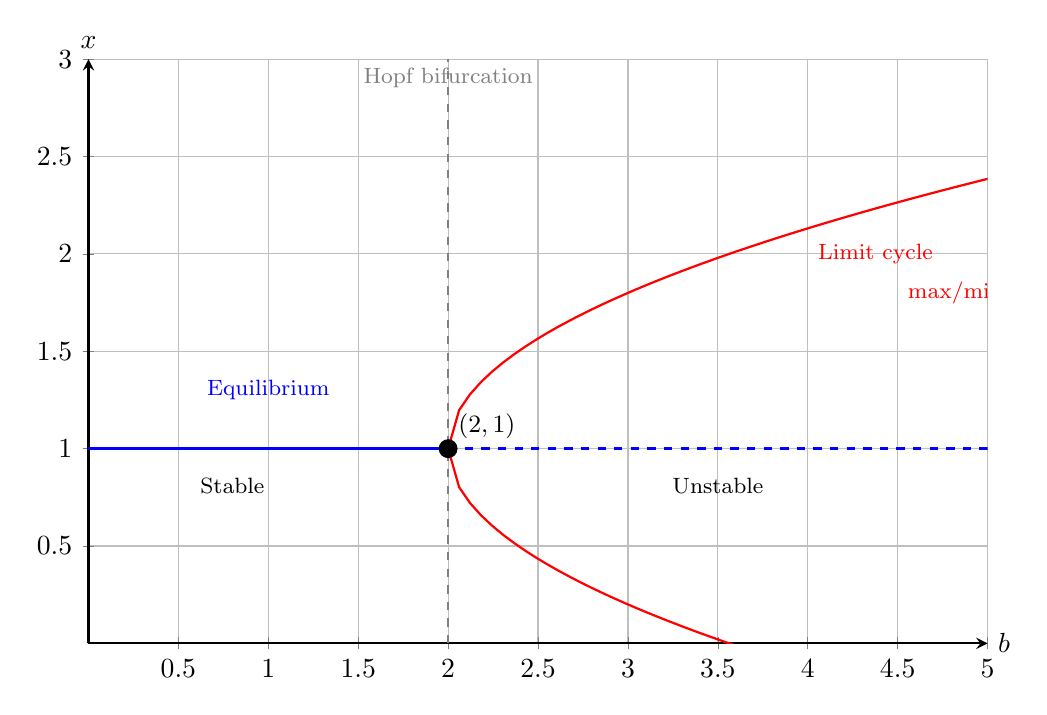
\begin{tikzpicture}
\begin{axis}[
    width=13cm,
    height=9cm,
    xlabel={$b$},
    ylabel={$x$},
    xmin=0, xmax=5,
    ymin=0, ymax=3,
    grid=major,
    axis lines=middle,
    thick,
    every axis x label/.style={at={(current axis.right of origin)},anchor=west},
    every axis y label/.style={at={(current axis.above origin)},anchor=south}
]

% Equilibrium x = 1 stable (b < 2)
\addplot[blue, very thick, solid, domain=0:2] {1};

% Equilibrium x = 1 unstable (b > 2)
\addplot[blue, very thick, dashed, domain=2:5] {1};

% Limit cycle envelope (schematic - grows from bifurcation)
% Upper envelope: x_max ≈ 1 + A*sqrt(b-2) for b > 2
% Lower envelope: x_min ≈ 1 - A*sqrt(b-2) for b > 2
\addplot[red, thick, domain=2:5, samples=50] {1 + 0.8*sqrt(x-2)};
\addplot[red, thick, domain=2:5, samples=50] {1 - 0.8*sqrt(x-2)};

% Bifurcation point
\addplot[mark=*, mark size=3pt, black, only marks] coordinates {(2, 1)};
\node[above right, font=\small] at (axis cs:2,1) {$(2, 1)$};

% Labels
\node[blue, anchor=south, font=\footnotesize] at (axis cs:1,1.2) {Equilibrium};
\node[anchor=north, font=\footnotesize] at (axis cs:0.8,0.9) {Stable};
\node[anchor=north, font=\footnotesize] at (axis cs:3.5,0.9) {Unstable};
\node[red, anchor=west, font=\footnotesize] at (axis cs:4,2) {Limit cycle};
\node[red, anchor=west, font=\footnotesize] at (axis cs:4.5,1.8) {max/min};

% Vertical line at bifurcation
\draw[gray, dashed] (axis cs:2,0) -- (axis cs:2,3);
\node[gray, anchor=south, font=\footnotesize] at (axis cs:2,2.8) {Hopf bifurcation};

\end{axis}
\end{tikzpicture}
\end{center}

\subsection*{Bifurcation diagram: $b$ vs $y$}

\begin{center}
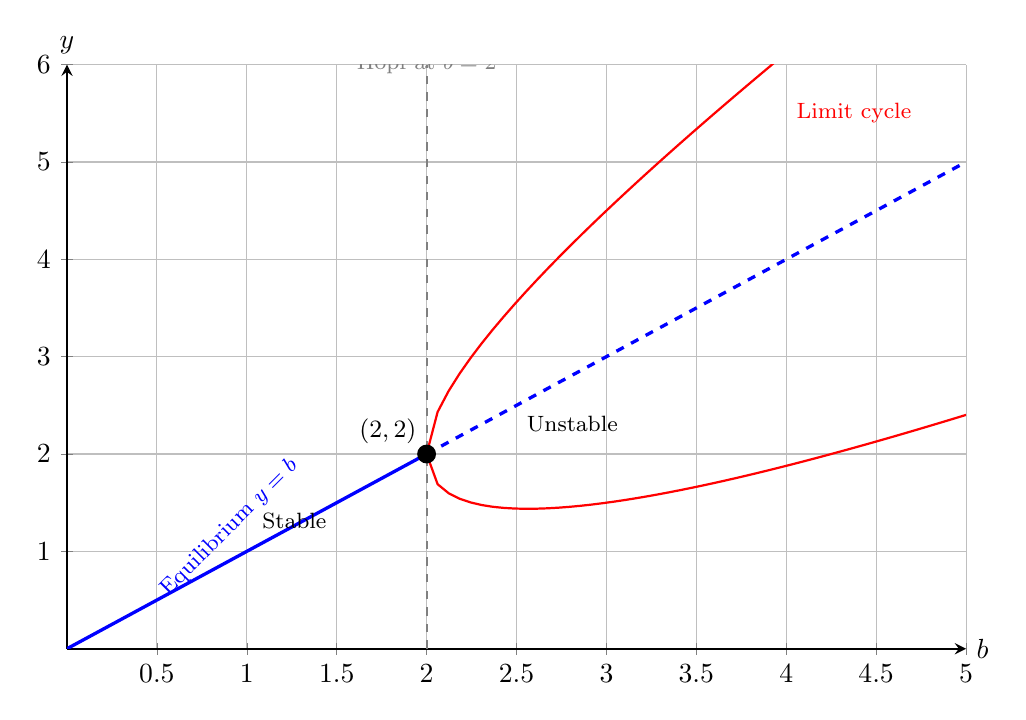
\begin{tikzpicture}
\begin{axis}[
    width=13cm,
    height=9cm,
    xlabel={$b$},
    ylabel={$y$},
    xmin=0, xmax=5,
    ymin=0, ymax=6,
    grid=major,
    axis lines=middle,
    thick,
    every axis x label/.style={at={(current axis.right of origin)},anchor=west},
    every axis y label/.style={at={(current axis.above origin)},anchor=south}
]

% Equilibrium y = b stable (b < 2)
\addplot[blue, very thick, solid, domain=0:2] {x};

% Equilibrium y = b unstable (b > 2)
\addplot[blue, very thick, dashed, domain=2:5] {x};

% Limit cycle envelope (schematic - oscillates around y = b)
% Upper envelope: y_max ≈ b + B*sqrt(b-2)
% Lower envelope: y_min ≈ b - B*sqrt(b-2)
\addplot[red, thick, domain=2:5, samples=50] {x + 1.5*sqrt(x-2)};
\addplot[red, thick, domain=2:5, samples=50] {x - 1.5*sqrt(x-2)};

% Bifurcation point
\addplot[mark=*, mark size=3pt, black, only marks] coordinates {(2, 2)};
\node[above left, font=\small] at (axis cs:2,2) {$(2, 2)$};

% Labels
\node[blue, anchor=west, font=\footnotesize, rotate=45] at (axis cs:0.5,0.5) {Equilibrium $y=b$};
\node[anchor=north east, font=\footnotesize] at (axis cs:1.5,1.5) {Stable};
\node[anchor=north west, font=\footnotesize] at (axis cs:2.5,2.5) {Unstable};
\node[red, anchor=west, font=\footnotesize] at (axis cs:4,5.5) {Limit cycle};

% Vertical line at bifurcation
\draw[gray, dashed] (axis cs:2,0) -- (axis cs:2,6);
\node[gray, anchor=south, font=\footnotesize] at (axis cs:2,5.8) {Hopf at $b=2$};

\end{axis}
\end{tikzpicture}
\end{center}

\subsection*{XYZ Analysis of Bifurcation Diagrams}

\begin{itemize}[leftmargin=*]
\item \stage{STAGE X (What the diagrams show):} A single equilibrium branch that changes from solid (stable) to dashed (unstable) at $b = 2$. For $b > 2$, two additional curves emerge representing the maximum and minimum values of oscillations on the limit cycle.

\item \stage{STAGE Y (Why this structure):}
\begin{itemize}
\item \textbf{Equilibrium branch}: Shows the fixed point position. In $(b,x)$ space, it's horizontal at $x=1$ because $x^* = 1$ is independent of $b$. In $(b,y)$ space, it's diagonal $y=b$ because $y^* = b$ increases with parameter.
\item \textbf{Limit cycle envelope}: After bifurcation, trajectories don't settle to equilibrium but instead approach a periodic orbit. The envelope shows the range of oscillation - how far from equilibrium the system swings. Near $b=2$, amplitude is small (envelope close to equilibrium). As $b$ increases, amplitude grows roughly like $\sqrt{b-2}$ (typical for supercritical Hopf).
\item \textbf{Pitchfork-like appearance in $y$ diagram}: The diagram in $(b,y)$ space resembles a supercritical pitchfork, but it's not - the outer branches represent extrema of a single periodic orbit, not separate equilibria. This visual similarity sometimes causes confusion.
\end{itemize}

\item \stage{STAGE Z (What dynamics look like):}
\begin{itemize}
\item \textbf{Below bifurcation ($b < 2$)}: Trajectories spiral inward to $(1,b)$ and stay there (steady state)
\item \textbf{At bifurcation ($b = 2$)}: Critical point; trajectories slowly circulate near $(1,2)$ but don't quite settle
\item \textbf{Above bifurcation ($b > 2$)}: Trajectories spiral outward from $(1,b)$ until reaching the limit cycle, then circulate on it indefinitely (sustained oscillations)
\item \textbf{Far above ($b \gg 2$)}: Large-amplitude oscillations; concentrations swing widely between max and min values
\end{itemize}
The bifurcation represents the onset of oscillatory behavior - a qualitative change from monotonic approach to periodic cycling.
\end{itemize}

\vspace{10pt}
\hrule
\vspace{10pt}

\section{Step 8: Summary of Brusselator Behavior}

\subsection*{System parameters}

With $a = q = p = 1$:
\begin{align*}
\dot{x} &= 1 - (b+1)x + x^2y \\
\dot{y} &= bx - x^2y
\end{align*}

\subsection*{Part (a): Equilibrium}

\[
\boxed{(x^*, y^*) = (1, b)} \quad \text{for all } b > 0
\]

Unique equilibrium exists for all positive reaction rates.

\subsection*{Part (b): Stability}

\textbf{Jacobian:}
\[
J(1,b) = \begin{pmatrix}
b - 1 & 1 \\
-b & -1
\end{pmatrix}
\]

\textbf{Eigenvalues:}
\begin{align*}
\tau &= b - 2 \\
\Delta &= 1 \\
\lambda &= \frac{b - 2}{2} \pm i\frac{\sqrt{4 - (b-2)^2}}{2} \quad \text{for } 0 < b < 4
\end{align*}

\textbf{Stability classification:}
\begin{itemize}
\item $0 < b < 2$: Stable spiral (equilibrium attracts)
\item $b = 2$: Neutral, purely imaginary eigenvalues $\lambda = \pm i$
\item $2 < b < 4$: Unstable spiral (equilibrium repels)
\item $b \geq 4$: Unstable (real eigenvalues)
\end{itemize}

\subsection*{Part (c): Bifurcation}

\[
\boxed{\text{HOPF BIFURCATION}}
\]

\textbf{Location:}
\[
b = 2, \quad (x, y) = (1, 2), \quad \text{i.e., } (x, y, b) = (1, 2, 2)
\]

\textbf{Characteristics:}
\begin{itemize}
\item Supercritical type (stable limit cycle emerges for $b > 2$)
\item Oscillation frequency at bifurcation: $\omega = 1$ (period $T = 2\pi$)
\item Amplitude near bifurcation: $A \propto \sqrt{b - 2}$
\end{itemize}

\textbf{Physical interpretation:}
\begin{itemize}
\item Below threshold ($b < 2$): Chemical reaction reaches steady-state concentrations
\item Above threshold ($b > 2$): Chemical oscillator - concentrations vary periodically
\item Critical value ($b = 2$): Onset of spontaneous oscillations
\end{itemize}

\textbf{Bifurcation diagrams:}
\begin{itemize}
\item In $(b, x)$ space: Horizontal equilibrium line at $x=1$ with limit cycle envelope growing from $b=2$
\item In $(b, y)$ space: Diagonal equilibrium line $y=b$ with limit cycle envelope (resembles pitchfork but represents oscillation amplitudes)
\end{itemize}

\subsection*{Connection to real chemistry}

The Brusselator models reactions like the Belousov-Zhabotinsky reaction where:
\begin{itemize}
\item Multiple chemical species interact autocatalytically
\item Continuous supply of reactants maintains far-from-equilibrium conditions
\item Concentrations spontaneously oscillate with visible color changes
\item Oscillation onset occurs when reaction rates exceed critical threshold
\end{itemize}

The Hopf bifurcation at $b=2$ represents the transition from chemical equilibrium to chemical oscillations - a beautiful example of self-organization in nonlinear dynamics.

\end{document}
